\documentclass[]{article}
%\usepackage{setspace}
%\onehalfspacing
\usepackage{amsmath,amssymb,amsthm}
\renewcommand{\qedsymbol}{$\blacksquare$}
\usepackage{amsmath}
\usepackage{amsfonts}
\usepackage{mathrsfs}
\usepackage{amssymb}
\usepackage{enumerate}
\usepackage{mdwlist}
\usepackage{dirtytalk}
%\usepackage(graphicx}
\usepackage{xparse}
\usepackage{physics}
\usepackage{graphicx}
\setcounter{MaxMatrixCols}{13}
\setlength\parindent{0pt}
\usepackage[none]{hyphenat}
\usepackage[hmarginratio=1:1]{geometry}
\begin{document}
%\begin{center}
{\Large Physics 614 Homework 1}\\
{Jeremy Welsh-Kavan}\\
%\end{center}
\vspace{0.2 cm}
\noindent\rule{15cm}{0.4pt} \\
\begin{enumerate}[1)]

\item {\bf Spin and rotational angular momentum: ortho/para Hydrogen }
\begin{enumerate}[i.]
\item To calculate the rotational partition function, $\mathcal{Z}_p$, we just sum the Boltzmann factors over the index of allowed angular momentum eigenstates for parahydrogen. For the Hamiltonian,
\begin{equation}
\mathcal{H} = \frac{\hbar^2}{2I}\ell(\ell+1) \textrm{,  } \ell = 0, 2, 4,...
\end{equation}
the rotational partition function is
\begin{equation}
\begin{split}
\mathcal{Z}_p & = \sum_{\ell \text{ even}}^{\infty} (2\ell +1)e^{-\frac{\beta \hbar^2}{2I}\ell(\ell+1)} \\
\mathcal{Z}_p & = \sum_{n=0}^{\infty} (4n +1)e^{-\frac{\beta \hbar^2}{2I}2n(2n+1)} \\
\mathcal{Z}_p & = \sum_{n=0}^{\infty} (4n +1)e^{-\frac{\theta_{\text{rot}}}{T}2n(2n+1)} \\
\end{split}
\end{equation}
where we have introduced a characteristic temperature scale, $\theta_{\text{rot}} := \frac{\hbar^2}{2k_B I}$. \\
\hfill \\
In the low temperature, $\theta_{\text{rot}} \gg T$, limit the exponential in (2) is small so the zeroth term dominates the sum. To first order, the rotational partition functions becomes \\
\begin{equation}
\begin{split}
\mathcal{Z}_p & \approx 1 + 5e^{-6\frac{\theta_{\text{rot}}}{T}} \\
\end{split}
\end{equation}
\hfill \\
In the high temperature, $\theta_{\text{rot}} \ll T$, limit the sum is well approximated by the integral of a smooth function
\begin{equation}
\begin{split}
\mathcal{Z}_p & \approx \int_{0}^{\infty} dx (4x +1)e^{-\frac{\theta_{\text{rot}}}{T}2x(2x+1)} \\
\mathcal{Z}_p & \approx \frac{T}{2\theta_{\text{rot}}} \\
\end{split}
\end{equation}
\item In orthohydrogen, the pair of nuclei can occupy $\ket{\uparrow\uparrow}$, $\ket{\downarrow\downarrow}$, and $\frac{1}{\sqrt{2}}( \ket{\uparrow\downarrow} + \ket{\downarrow\uparrow} )$ so each angular momentum eigenstate has an additional triple degeneracy. The rotational partition function for orthohydrogen is therefore
\begin{equation}
\begin{split}
\mathcal{Z}_o & = \sum_{\ell \text{ odd}}^{\infty} 3(2\ell +1)e^{-\frac{\theta_{\text{rot}}}{T}\ell(\ell+1)} \\
\mathcal{Z}_o & = 3\sum_{n=0}^{\infty} (4n+3)e^{-\frac{\theta_{\text{rot}}}{T}(2n+1)(2n+2)} \\
\mathcal{Z}_o & \approx 9e^{-2\frac{\theta_{\text{rot}}}{T}} \text{, for }  \theta_{\text{rot}} \gg T\\
\mathcal{Z}_o & \approx \frac{3T}{2\theta_{\text{rot}}}e^{-2\frac{\theta_{\text{rot}}}{T}} \text{, for }  \theta_{\text{rot}} \ll T\\
\end{split}
\end{equation}
\item The sum of the two partition functions above is the total rotational partition function for hydrogen. The number of each configuration is just the nubmer of particles $N$ multiplied by the probability of being in either configuration. \\
\begin{equation}
\begin{split}
n_o & = N \frac{\mathcal{Z}_o}{\mathcal{Z}_o + \mathcal{Z}_p} \\
n_p & = N \frac{\mathcal{Z}_p}{\mathcal{Z}_o + \mathcal{Z}_p} \\
\end{split}
\end{equation}
And the proportion of particles in the orthohydrogen state to particles in the parahydrogen state is just the ratio $n_o/n_p$.
\begin{equation}
\begin{split}
\frac{n_o}{n_p} & = \frac{\mathcal{Z}_o}{\mathcal{Z}_p}
\end{split}
\end{equation}
In the low temperature limit, 
\begin{equation}
\begin{split}
\frac{n_o}{n_p} & \approx \frac{9e^{-2\frac{\theta_{\text{rot}}}{T}} }{1 + 5e^{-6\frac{\theta_{\text{rot}}}{T}} } \\
& \approx 9e^{-2\frac{\theta_{\text{rot}}}{T}} \\
\end{split}
\end{equation}
And in the high temperature limit,
\begin{equation}
\begin{split}
\frac{n_o}{n_p} & \approx 3e^{-2\frac{\theta_{\text{rot}}}{T}} \\
& \approx 3 \\
\end{split}
\end{equation}
\item For an equilibrium ideal gas of $N$ particles, each with rotational partition function $\mathcal{Z}_\text{rot} = \mathcal{Z}_o + \mathcal{Z}_p$, the rotational partition function for the whole system is
\begin{equation}
\begin{split}
\mathcal{Z} & = \frac{\mathcal{Z}_\text{rot}^N}{N!} \\
\end{split}
\end{equation}
To compute the rotational contribution to the heat capacity, we first calculate the following quantities
\begin{equation}
\begin{split}
F & = -k_B T \ln \left( \mathcal{Z}\right)\\
S & = - \left( \pdv{F}{T}\right)_{N,V}\\
\end{split}
\end{equation}
In the low temperature limit,
\begin{equation}
\begin{split}
F & = -Nk_B T \ln \left( 1 + 9e^{-2\frac{\theta_{\text{rot}}}{T}}\right) - k_BT \ln(N!)\\
& \approx -9Nk_B T  e^{-2\frac{\theta_{\text{rot}}}{T}} -k_BT\left(  N\ln(N) - N \right) \\
S & = 9Nk_B\left(  1 + \frac{2 \theta_{\text{rot}}}{T} \right)  e^{-2\frac{\theta_{\text{rot}}}{T}}   -Nk_B\left(  \ln(N) - 1 \right)  \\
C& = T \left( \pdv{S}{T}\right)_{N} \\
\implies C & = \frac{36Nk_B\theta_\text{rot}^2}{T^2}e^{-2\frac{\theta_{\text{rot}}}{T}}  \\ 
\end{split}
\end{equation}
In the high temperature limit, 
\begin{equation}
\begin{split}
F & = -Nk_B T \ln \left( \frac{T}{2\theta_{\text{rot}}}   +  \frac{3T}{2\theta_{\text{rot}}}e^{-2\frac{\theta_{\text{rot}}}{T}} \right) - k_BT \ln(N!)\\
& = -Nk_B T \left(   \ln( \frac{T}{2\theta_\text{rot}}) + \ln(1+ 3e^{-2\frac{\theta_{\text{rot}}}{T}}) \right) - k_BT \ln(N!)\\
& \approx -Nk_B T \left(   \ln( \frac{T}{2\theta_\text{rot}}) + 3e^{-2\frac{\theta_{\text{rot}}}{T}} \right) - k_BT \ln(N!)\\
S & = \text{Nk} \left(e^{-\frac{2 \theta }{T}} \left(\frac{6 \theta }{T}+3\right)+\log \left(\frac{T}{2 \theta }\right)+1\right)\\ 
\implies C & = Nk_B + \frac{12Nk_B\theta_\text{rot}^2}{T^2} e^{-2\frac{\theta_{\text{rot}}}{T}} \\
C & \approx Nk_B \\
\end{split}
\end{equation}
\item Starting with the full expression for $Z_\text{rot}$ as an infinite sum, we numerically calculate and plot $C_V/Nk_B$ as a function $T/\theta_\text{rot}$. \\
\begin{equation}
\begin{split}
C_V & = T\left( \pdv[2]{F}{T} \right)_{N,V} \\
C_V & = Nk_BT\pdv[2]{T}\left( T\ln(   \mathcal{Z}_o +       \mathcal{Z}_p      ) \right) \\
C_V & = Nk_BT\pdv[2]{T}\left(T \ln(   \sum_{n=0}^{\infty} 3(4n+3)e^{-\frac{\theta_{\text{rot}}}{T}(2n+1)(2n+2)} 
+ (4n +1)e^{-\frac{\theta_{\text{rot}}}{T}2n(2n+1)}  ) \right)\\
\frac{C_V}{Nk_B} & = T\pdv[2]{T}\left( T \ln(   \sum_{n=0}^{\infty} 3(4n+3)e^{-\frac{\theta_{\text{rot}}}{T}(2n+1)(2n+2)} 
+ (4n +1)e^{-\frac{\theta_{\text{rot}}}{T}2n(2n+1)}  ) \right)\\
\frac{C_V}{Nk_B} & = \tau \pdv[2]{\tau}\left( \tau \ln(   \sum_{n=0}^{\infty} 3(4n+3)e^{-\frac{1}{\tau}(2n+1)(2n+2)} 
+ (4n +1)e^{-\frac{1}{\tau}2n(2n+1)}  ) \right)\\
\end{split}
\end{equation}
where we have defined $\tau := T/\theta_\text{rot}$. \\
Below is a plot, generated using Mathematica, of
\begin{equation}
\begin{split}
\frac{C_V}{Nk_B} & = \tau \pdv[2]{\tau}\left( \tau \ln(   \sum_{n=0}^{N} 3(4n+3)e^{-\frac{1}{\tau}(2n+1)(2n+2)} 
+ (4n +1)e^{-\frac{1}{\tau}2n(2n+1)}  ) \right)\\
\end{split}
\end{equation}
for different values of $N$. The maximum value of $N$ shown is $N=3$ because plots using greater values of $N$ are not visibly different from $N=3$ on this temperature scale. Apologies, I couldn't get the plot to show up in the right place.\\
\begin{figure}[h]
	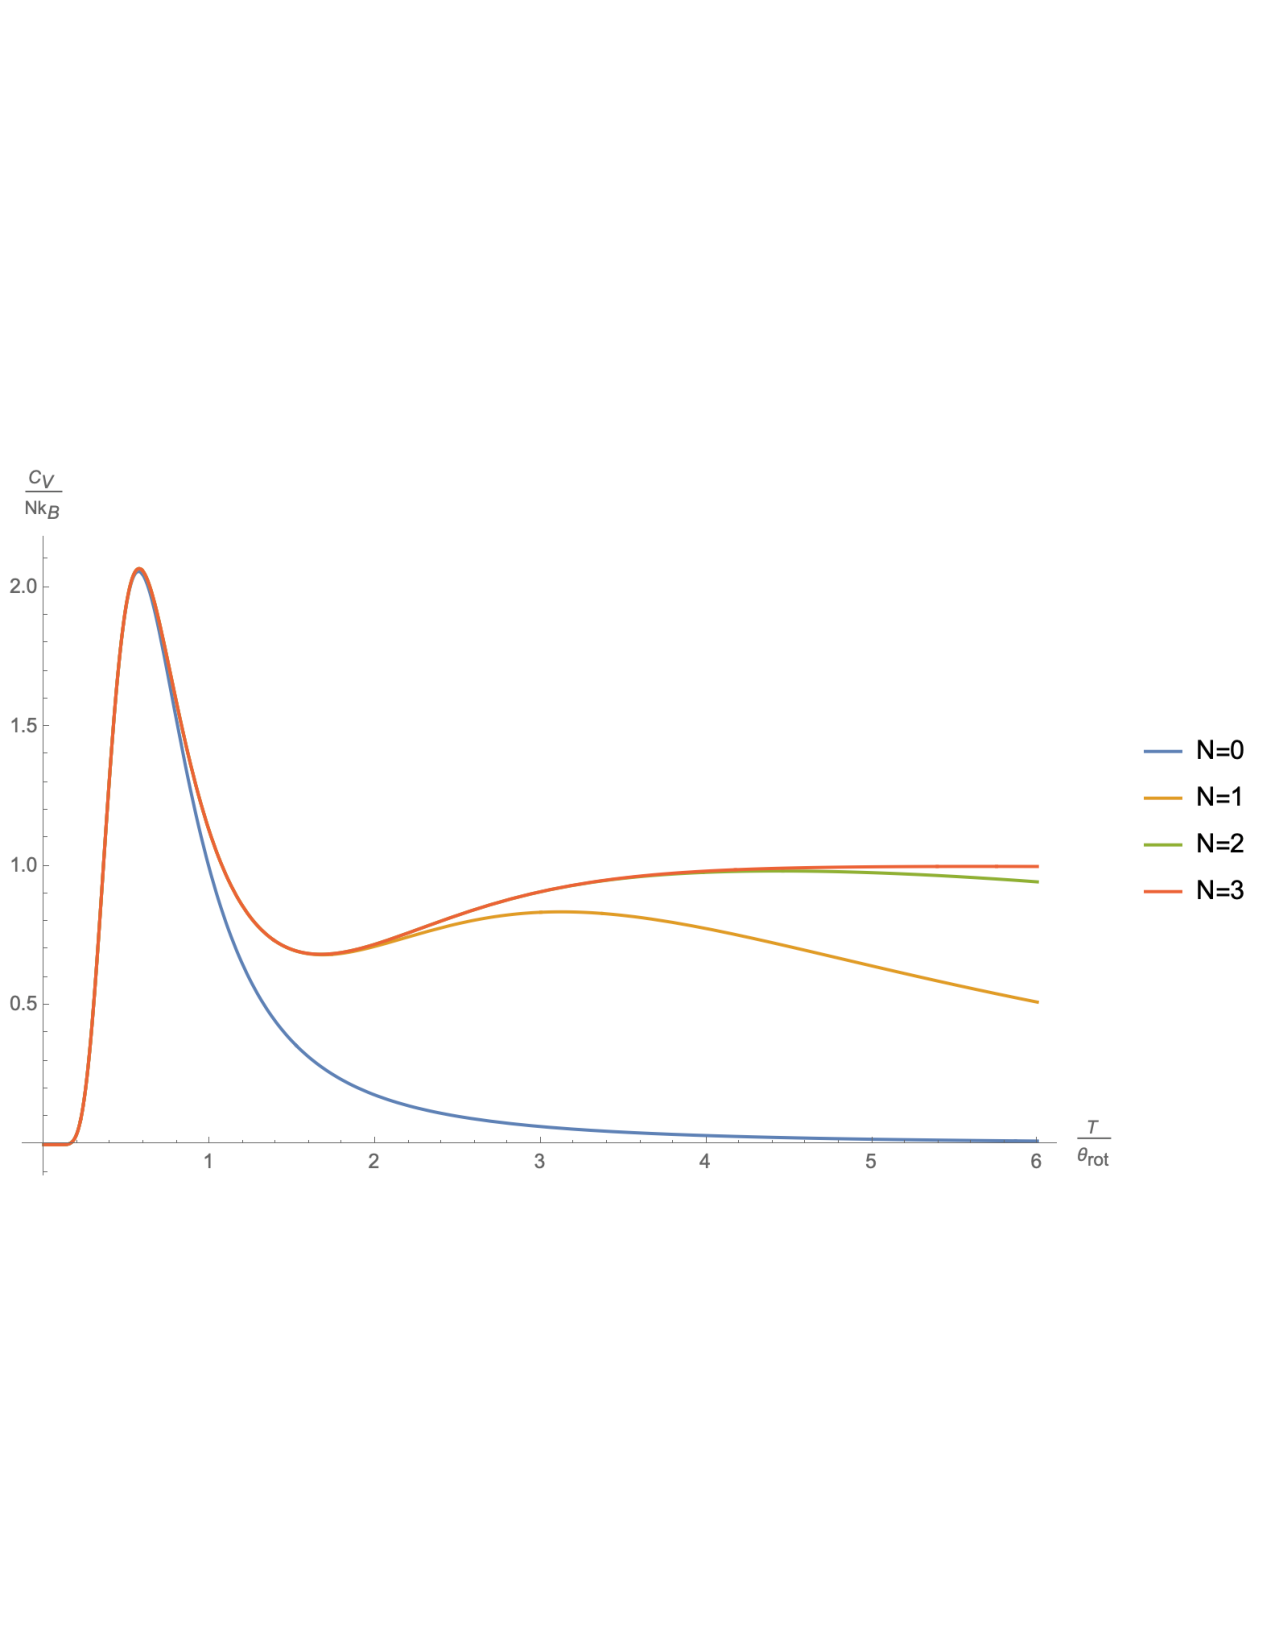
\includegraphics[trim = 0in 1.4in 0in 1.4in,clip, width=6.5in]{CVplot.pdf}
	\caption{A plot of $C_V/Nk_B$ for four values of $N$.}
\end{figure}


\end{enumerate}
\item {\bf Density matrix example: photons}
\begin{enumerate}[i)]
\item A pure state is a state whose density matrix, $\rho$, satisfies $\text{tr}\left(\rho^2 \right)=1$. We claim that a density matrix $\rho$ corresponds to a pure state if and only if $\rho^2=\rho$. \\
\begin{proof} \hfill\\
\begin{enumerate}[I.]
\item Suppose $\rho$ corresponds to a pure state. Then we can write $\rho$ in terms of a single state vector, $\ket{\psi}$, as $\rho = \ket{\psi}\bra{\psi}$. In which case, $\rho^2 = \ket{\psi}\bra{\psi}\ket{\psi}\bra{\psi} = \bra{\psi}\ket{\psi}\ket{\psi}\bra{\psi} = \rho$, since $\bra{\psi}\ket{\psi} = 1$. Therefore, if $\rho$ corresponds to a pure state, then $\rho = \rho^2$. \\
\item Now suppose $\rho$ is a density matrix such that $\rho^2 = \rho$. Then $\text{tr}\left(\rho^2\right) = \text{tr}\left(\rho \right)$. Since $\rho$ is a density matrix, we must have $\text{tr}\left(\rho \right)=1$. So $\text{tr}\left(\rho^2\right) = \text{tr}\left(\rho \right)=1$. Therefore, if $\rho$ is a density matrix satisfying $\rho^2 = \rho$, then $\rho$ corresponds to a pure state. \\
\end{enumerate}
\end{proof}
\item Let vertical polarization, $\ket{V}$, correspond to $\mqty(1 \\ 0)$ and let horizontal polarization, $\ket{H}$, correspond to $\mqty(0 \\ 1)$. \\
\begin{itemize}
\item If $\rho$ corresponds to a vertically polarized photon in the pure state $\ket{V}$ then

\begin{equation}
\begin{split}
\rho & = \mqty(1 \\ 0)\mqty(1 & 0) \\ 
\rho & = \mqty(1  & 0 \\ 0 & 0) \\ 
\end{split}
\end{equation}
\item If $\rho$ corresponds to a diagonally polarized photon in the pure state $\frac{1}{\sqrt{2}}\left( \ket{V} + \ket{H}\right)$, then

\begin{equation}
\begin{split}
\rho & = \frac{1}{2} \left(\mqty(1 \\ 0) + \mqty( 0 \\ 1) \right) \left( \mqty(1 & 0) + \mqty( 0 & 1)\right) \\
\rho & = \frac{1}{2} \left(\mqty(1 & 0 \\  0 & 0) + \mqty( 0 & 0 \\ 1 & 0) + \mqty( 0 & 1 \\ 0  & 1) + \mqty( 0 & 0 \\ 0 & 1)\right) \\
\rho & = \frac{1}{2} \mqty(1 & 1 \\  1 & 1)  \\
\end{split}
\end{equation}

\item If $\rho$ corresponds to unpolarized light, i.e. a mixed state of vertical and horizontal polarization in equal proportions, then 

\begin{equation}
\begin{split}
\rho & = \frac{1}{2} \ket{V}\bra{V} + \frac{1}{2}\ket{H}\bra{H} \\
\rho & = \frac{1}{2} \mqty( 1 & 0 \\ 0& 1) \\
\end{split}
\end{equation}

\end{itemize}


\item We compute $\text{tr}\left(\rho\right)$, $\text{tr}\left(\rho^2\right)$, and the von Neumann entropy $S = -k_B\text{tr}\left(\rho\log\rho\right)$ for each of the density matrices in ii).  We will use the fact that, if $\rho$ can be written in terms of its eigenvectors $\ket{\alpha}$ as $\rho=\sum_{\alpha}\lambda_\alpha\ket{\alpha}\bra{\alpha}$, then $S = -k_B\sum_{\alpha}\lambda_\alpha \ln\lambda_\alpha$. \footnote{en.wikipedia.org/wiki/Von\_Neumann\_entropy} \\
\begin{itemize}

\item $\rho = \mqty( 1 & 0 \\ 0 & 0 )$, $\rho^2 = \mqty( 1 & 0 \\ 0 & 0 ) $
\begin{equation}
\begin{split}
\text{tr}\left(\rho\right) &= 1 \\
\text{tr}\left(\rho^2\right) &= 1 \\
S & = 0 \\
\end{split}
\end{equation}

\item $\rho = \frac{1}{2} \mqty(1 & 1 \\  1 & 1)$, $\rho^2 = \frac{1}{2}\mqty( 1 & 1 \\ 1 & 1 ) $ In this case, the eigenvectors of $\rho$ are $\mqty( 1 \\1 )$ and $\mqty( 1 \\ -1 )$ with eigenvalues $1$ and $0$ respectively. \\
\begin{equation}
\begin{split}
\text{tr}\left(\rho\right) &= 1 \\
\text{tr}\left(\rho^2\right) &= 1 \\
S & = 0 \\
\end{split}
\end{equation}

\item $\rho  = \frac{1}{2} \mqty( 1 & 0 \\ 0& 1) $, $\rho^2  = \frac{1}{4} \mqty( 1 & 0 \\ 0& 1) $\\
\begin{equation}
\begin{split}
\text{tr}\left(\rho\right) &= 1 \\
\text{tr}\left(\rho^2\right) &= \frac{1}{2} \\
S & = k_B\ln 2 \\
\end{split}
\end{equation}

\end{itemize}

We find that the von Neumann entropy of a system is lowest in a pure state and higher in a mixed state. The Wikipedia article cited below states that the von Neumann entropy ``quantifies the departure of the system from a pure state". By inspection and some guessing, the von Neumann entropy seems like, in some sense, it measures the dimension of the subspace of the available Hilbert space occupied by the system. \\

\end{enumerate}
\noindent\rule{15cm}{0.4pt} \\
\item {\bf Canonical density matrix: electron spin} \\
\\
\hfill
$\mathcal{H} = -\mu_B\vec{\sigma}\cdot\vec{B}$, $\sigma_x=\mqty(0&1\\1&0)$, $\sigma_y=\mqty(0&-i\\i&0)$, $\sigma_z=\mqty(1&0\\0&-1)$
\begin{enumerate}[a)]

\item  {\bf Proposition:} Each Pauli matrix, $\sigma_i$, satisfies $e^{a\sigma_i} = \cosh(a\textbf{I}) + \sinh(a\sigma_i) = \cosh(a)\textbf{I} + \sinh(a)\sigma_i $. 
\begin{proof}
Beginning with the power series for $e^{a\sigma_i}$, we have
\begin{equation}
\begin{split}
e^{a\sigma_i} & = \sum_{n=0}^{\infty} \frac{(a\sigma_i)^n}{n!} \\
e^{a\sigma_i} & = \sum_{n \text{ even}}^{\infty} \frac{(a\sigma_i)^n}{n!} + \sum_{n \text{ odd}}^{\infty} \frac{(a\sigma_i)^n}{n!}  \\ 
e^{a\sigma_i} & = \sum_{n \text{ even}}^{\infty} \frac{(a\textbf{I})^n}{n!} + \sum_{n \text{ odd}}^{\infty} \frac{(a\sigma_i)^n}{n!}  \\ 
\implies e^{a\sigma_i} & = \cosh(a\textbf{I}) + \sinh(a\sigma_i) \\
e^{a\sigma_i} & = \sum_{n \text{ even}}^{\infty} \textbf{I}\frac{a^n}{n!} + \sum_{n \text{ odd}}^{\infty} \sigma_i\frac{a^n}{n!}  \\ 
\implies e^{a\sigma_i} & = \cosh(a)\textbf{I} + \sinh(a)\sigma_i \\
\end{split}
\end{equation}
Where we have used the fact that $\sigma_i^n = \textbf{I}$ if $n$ is even and $\sigma_i^n=\sigma_i$ if $n$ is odd.
\end{proof} 
\hfill \\
If $\vec{B}=B\hat{z}$, then $\mathcal{H}=-\mu_BB\sigma_z$. In the quantum canonical ensemble $\rho$ is given by

\begin{equation}
\rho = \frac{   e^{-\beta\mathcal{H}}   }{\text{tr}\left(  e^{-\beta\mathcal{H}}   \right)}
\end{equation}
Therefore, we have 

\begin{equation}
\begin{split}
\rho & = \frac{   e^{\beta\mu_BB\sigma_z}   }{\text{tr}\left(  e^{\beta\mu_BB\sigma_z}   \right)} \\
\rho & = \frac{   \cosh(\beta\mu_BB)\textbf{I} + \sinh(\beta\mu_BB)\sigma_z }{\text{tr}\left(   \cosh(\beta\mu_BB)\textbf{I} + \sinh(\beta\mu_BB)\sigma_z\right)} \\
\rho & = \frac{   \cosh(\beta\mu_BB)\textbf{I} + \sinh(\beta\mu_BB)\sigma_z }{\cosh(\beta\mu_BB)\text{tr}\left(   \textbf{I} \right)  + \sinh(\beta\mu_BB)\text{tr}\left(\sigma_z\right)} \\
\rho & = \frac{   \cosh(\beta\mu_BB)\textbf{I} + \sinh(\beta\mu_BB)\sigma_z }{2\cosh(\beta\mu_BB)}  \\
\rho & = \frac{1}{2}\textbf{I} + \frac{1}{2}\tanh(\beta\mu_BB)\sigma_z      \\
\rho & = \frac{1}{2}\mqty( 1 +   \tanh(\beta\mu_BB) & 0 \\ 0 & 1 -  \tanh(\beta\mu_BB)     ) \\
\end{split}
\end{equation}
\item If $\vec{B}=B\hat{x}$, then $\mathcal{H}=-\mu_BB\sigma_x$ and we have

\begin{equation}
\begin{split}
\rho & = \frac{   e^{\beta\mu_BB\sigma_x}   }{\text{tr}\left(  e^{\beta\mu_BB\sigma_x}   \right)} \\
\rho & = \frac{   \cosh(\beta\mu_BB)\textbf{I} + \sinh(\beta\mu_BB)\sigma_x }{\text{tr}\left(   \cosh(\beta\mu_BB)\textbf{I} + \sinh(\beta\mu_BB)\sigma_x\right)} \\
\rho & = \frac{1}{2} \left(    \textbf{I} +  \tanh(\beta\mu_BB)\sigma_x   \right) \\ 
\rho & = \frac{1}{2} \mqty( 1 &  \tanh(\beta\mu_BB) \\ \tanh(\beta\mu_BB) & 1    )     \\
\end{split}
\end{equation}

\item The average energy is just the expectation value of energy

\begin{enumerate}[a)]
\item
\begin{equation}
\begin{split}
\big< E \big> &= \text{tr}\left( \rho\mathcal{H}\right) \\
\big< E \big> &= \text{tr}\left(-\mu_BB \frac{1}{2}\mqty( 1 +   \tanh(\beta\mu_BB) & 0 \\ 0 & 1 -  \tanh(\beta\mu_BB)  )\mqty(1 & 0\\ 0 & -1)\right) \\
\big< E \big> &= - \frac{\mu_BB}{2}\text{tr}\left(   \mqty( 1 +   \tanh(\beta\mu_BB) & 0 \\ 0 &   \tanh(\beta\mu_BB) -1 )\right) \\
\big< E \big> &= - \mu_BB\tanh(\beta\mu_BB)
\end{split}
\end{equation}

\item
\begin{equation}
\begin{split}
\big< E \big> &= \text{tr}\left( \rho\mathcal{H}\right) \\
\big< E \big> &= \text{tr}\left(-\mu_BB \frac{1}{2}\mqty( 1 &  \tanh(\beta\mu_BB)  \\ \tanh(\beta\mu_BB)   & 1   )\mqty(0 & 1\\ 1 & 0)\right) \\
\big< E \big> &= - \frac{\mu_BB}{2}\text{tr}\left(   \mqty(  \tanh(\beta\mu_BB) & 1 \\ 1 &   \tanh(\beta\mu_BB)  )\right) \\
\big< E \big> &= - \mu_BB\tanh(\beta\mu_BB)
\end{split}
\end{equation}

\end{enumerate}
\end{enumerate}

\end{enumerate}
\noindent\rule{15cm}{0.4pt} \\
$$\clubsuit$$
\end{document}
%\begin{figure}[h]
%	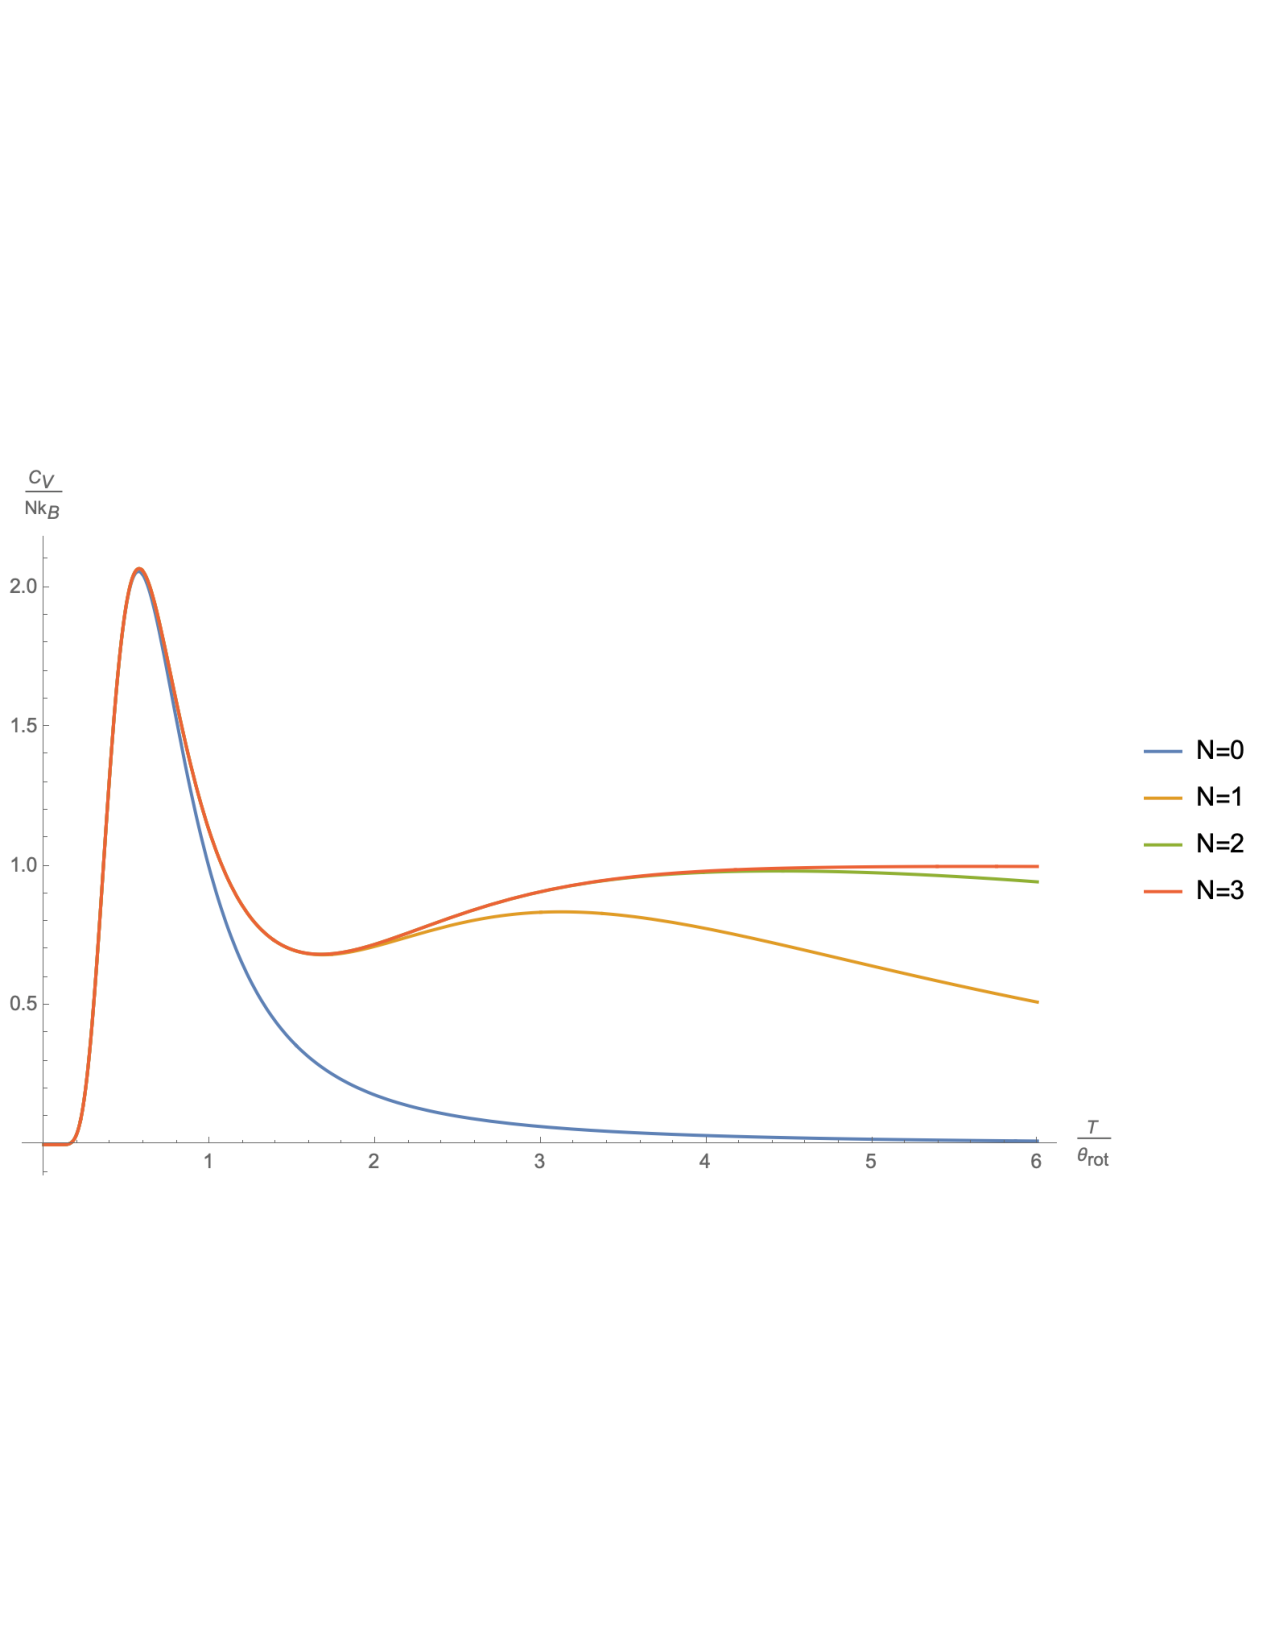
\includegraphics[trim = 0in 1.4in 0in 1.4in,clip, width=6.5in]{CVplot.pdf}
%	\caption{A graphical representation of the micro-canonical ensemble.}
%\end{figure}











%\begin{equation}
%\begin{split}
%\end{split}
%\end{equation}
